\documentclass[12pt]{article} % use larger type; default would be 10pt
\usepackage[utf8]{inputenc} % set input encoding (not needed with XeLaTeX)

%%% PAGE DIMENSIONS
\usepackage{geometry} % to change the page dimensions
\geometry{letterpaper} % or letterpaper (US) or a5paper or....
 \geometry{margin=1in} % for example, change the margins to 2 inches all round
% \geometry{landscape} % set up the page for landscape
%   read geometry.pdf for detailed page layout information

%%% PACKAGES
\usepackage{graphicx} % support the \includegraphics command and options
\usepackage{setspace}
\doublespacing
\usepackage[parfill]{parskip} % Activate to begin paragraphs with an empty line rather than an indent
\usepackage{booktabs} % for much better looking tables
\usepackage{array} % for better arrays (eg matrices) in maths
\usepackage{paralist} % very flexible & customisable lists (eg. enumerate/itemize, etc.)
\usepackage{verbatim} % adds environment for commenting out blocks of text & for better verbatim
\usepackage{subfig} % make it possible to include more than one captioned figure/table in a single float
% These packages are all incorporated in the memoir class to one degree or another...
\usepackage{amsmath} %Allow math
\usepackage{appendix} %Allow for creation of appendicies
\usepackage{textgreek} %Allow greek text outside math mode

%Allow big first letter in Paragraph
\usepackage{type1cm}
\usepackage{lettrine}

%DEFINE VARIABLES
\newcommand{\classnumber}{AAE\:412\:-\:Team\:32:}
\newcommand{\reportnumber}{Final Project}
\newcommand{\TAname}{Dr. Gregory Blaisdell}

%%% HEADERS & FOOTERS
\usepackage{fancyhdr} % This should be set AFTER setting up the page geometry
\pagestyle{fancy} % options: empty , plain , fancy
\renewcommand{\headrulewidth}{0pt} % customise the layout...
\lhead{}\chead{}\rhead{}
\lfoot{}\cfoot{\thepage\\Purdue University}\rfoot{}

%%% SECTION TITLE APPEARANCE
\usepackage{sectsty}
\allsectionsfont{\fontsize{12}{15}\centering\textbf} % (See the fntguide.pdf for font help)
\renewcommand{\thesection}{\Roman{section}.} 
\renewcommand{\thesubsection}{\textbf{\Alph{subsection}.}}
% (This matches ConTeXt defaults)
\usepackage[font=small,labelfont=bf]{caption} % Required for specifying captions to tables and figures

\renewcommand{\appendixname}{APPENDIX} %Change  Appendix Title to spell out the word

%%% END Article customizations

%%%MATLAB CODE
\usepackage[numbered,framed]{matlab-prettifier}
\renewcommand*{\lstlistlistingname}{List of MATLAB Code Snippets} %Change MATLAB ToC Title


%%% The "real" document content comes below...

\title{\classnumber\:\reportnumber}
\author{Jay Blake\\Devin Eubanks\\Brad Lock\\Purdue University}

\begin{document}
\maketitle
\vspace{2in}
\begin{center}
    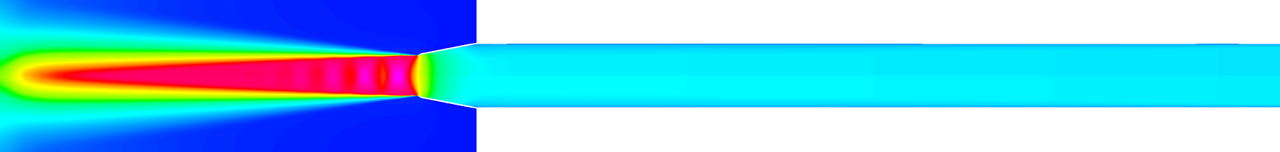
\includegraphics[width=\linewidth]{CoverPicture.png}
\end{center}
\clearpage
\begin{center}
{\Large\textbf{\classnumber\:\reportnumber}}\\
\vspace*{24pt}
Jay Blake\footnote{Engineer, School of Aeronautics and Astronautics, 701 W Stadium Ave, West Lafayette, IN 47907}, Devin M. Eubanks\footnote{Engineer, School of Aeronautics and Astronautics, 701 W Stadium Ave, West Lafayette, IN 47907}, and Bradley W. Lock\footnote{Engineer, School of Aeronautics and Astronautics, 701 W Stadium Ave, West Lafayette, IN 47907}\\
\textit{Purdue University, West Lafayette, IN, 47907}
\end{center}
\vspace*{48pt}
%Abstract
\textbf{\hspace{36pt}A Computational Fluid Dynamics simulation was ran on three nozzle geometries, defined by M. T.. Trumper, P. Behrouzi, and J. J. Mcguirk in \textit{Influence  of  nozzle  exit  conditions on  the  near-field  development  of  high  subsonic  and  underexpanded  axisymmetric  jets}. Analysis was performed on boundary layer and jet plume properties for supersonic conditions using a Nozzle Pressure Ratio of 2.2. An additional analysis was performed on one of the nozzles to determine flow properties of jet exhaust rather than air.}
\vspace*{36pt}
\section*{Nomenclature}
\begin{table}[ht]
    %\centering
    \begin{tabular}{l c l}
       $\alpha$&=&Angle of Attack\\
       CFD&=&Computational Fluid Dynamics\\
         M&=&Mach Number\\
         NPR&=&Nozzle Pressure Ratio\\
         $p$&=&Pressure\\
         $p_0$&=&Stagnation Pressure\\
         $p_a$&=&Atmospheric Pressure\\
         V&=&Velocity
    \end{tabular}
    \label{tab:nomenclature}
\end{table}

\section{Introduction}
\subsection{Experimental Motivation and Background}
\lettrine{A}{s} outlined in the paper by Trumper, et al., researchers set out to gain detailed knowledge of near field flow and jet plume development for different converging nozzle geometries.\cite{MilesT.Trumper2018IoNE} The goal was to use this data to work to reduce jet noise for civilian applications and infrared signature for military purposes. The experimental set up is shown in Figure \ref{fig:Setup}. It consisted of a high-pressure nozzle capable of air mass flow up to 0.8 kg/s at a maximum gauge pressure of 13.8 Bar. The flow could be intercooled and dried guaranteeing consistent flow between runs. The air was piped into the facility before passing through a 4:1 contraction into the final delivery pipe with a diameter of 75mm. This pipe could be fitted with several different test nozzles, the geometry of which will be discussed in the following subsection. In the experiment 4 geometries at NPRs ranging from 1.3 to 2.4 were used. This provided both high-subsonic and supersonic flows with the critical NPR being 1.893 for air.

\begin{center}
    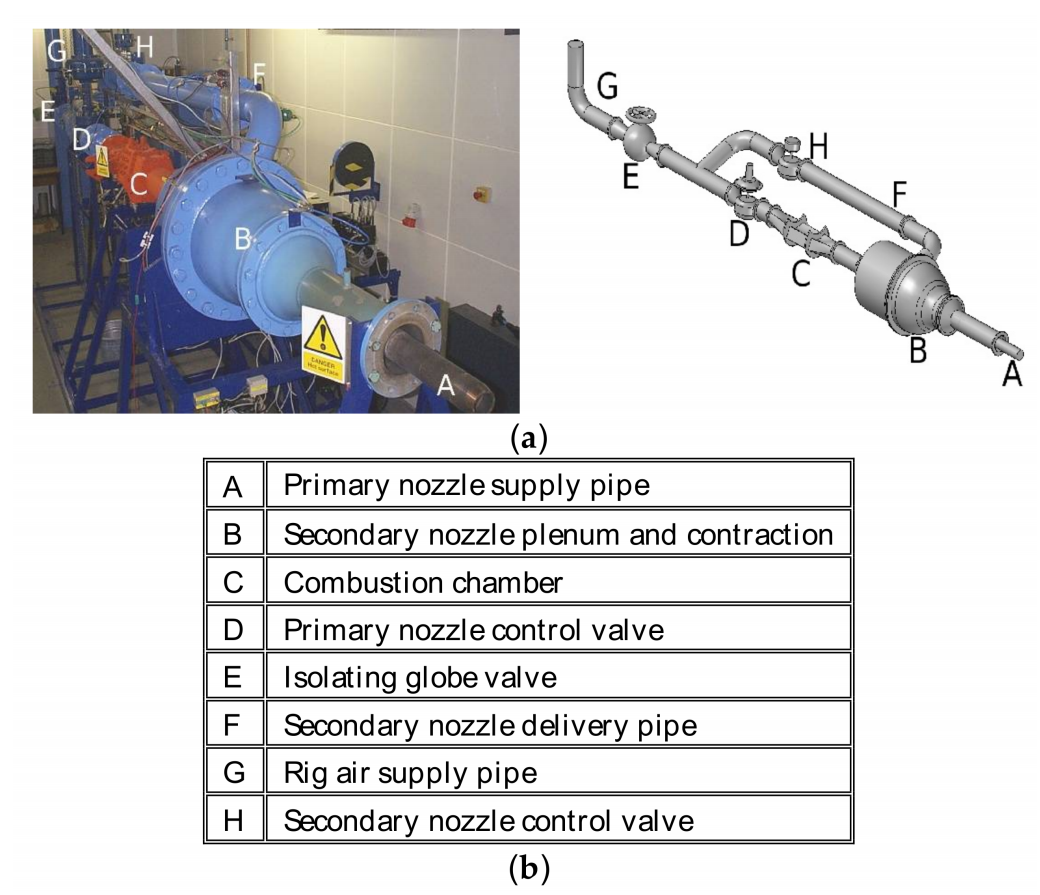
\includegraphics[width = 4in]{setup.PNG}
    \captionof{figure}{Experimental Setup}
    \label{fig:Setup}
\end{center}

\subsection{Project Motivation and Problem Definition}
The overarching motivation behind this project is to competently model real-world experimental results using CFD. The tests described above were modeled computationally and results compared to check the validity of the model. Further, analysis was done and conclusions drawn based on the data received to extend the scope of the experimental results. 

Three specific cases were chosen to model computationally against the experiment. The three cases include running flow through three of the four nozzle geometries provided all at an NPR of 2.2. This NPR was chosen because it is well above the critical pressure ratio, guaranteeing that flow will reach supersonic conditions. The three nozzles used were LU48(Nozzle A), LU60(Nozzle B), and LU48P(Nozzle C) as shown in figure \ref{fig:geometries}. Respectively these nozzles converged to a 48mm diameter exit, 60mm diameter, and a 48mm diameter, but with a flat portion at the exit of length 35mm. A main point of focus in this project is to examine the effect of the flat extension on the jet plume and flow field. 

\begin{center}
    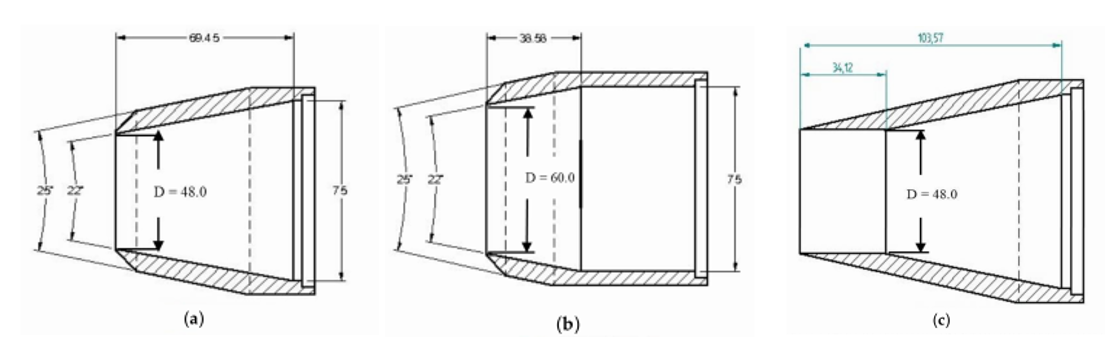
\includegraphics[width = \linewidth]{Geometries.png}
    \captionof{figure}{Geometries Modeled}
    \label{fig:geometries}
\end{center}

\section{Numerical Solution}
\subsection{Geometry}
ANSYS Fluent was used to develop a numerical solution for Nozzles (a), (b), and (c) shown in Figure \ref{fig:geometries}. For each nozzle, Design Modeler was used to create the geometry. In the paper written by Trumper, et al., it was noted that the first 10-15 exit diameters around the output of a jet are important in the analysis of jet plumes \cite{MilesT.Trumper2018IoNE}, so the outer domain was defined out to 20 exit diameters for each case. The inlet pipe length was chosen such that the boundary layer at the nozzle inlet was 29mm, matching the boundary layer defined in the paper. The domains used are shown with meshing in Section \ref{section:mesh}\par

In order to determine the pipe length required to reach the proper boundary layer, the pipe was extended to 2 meters and ran in Fluent using the boundary conditions in Table \ref{tab:boundary}. Then, CFD Post was used to show the Mach contours and the location within the pipe was found visually to be 1.21 meters from the inlet, as shown in Figure \ref{fig:boundarylength}. The pipe was then shortened to this length in all geometries.

\begin{center}
    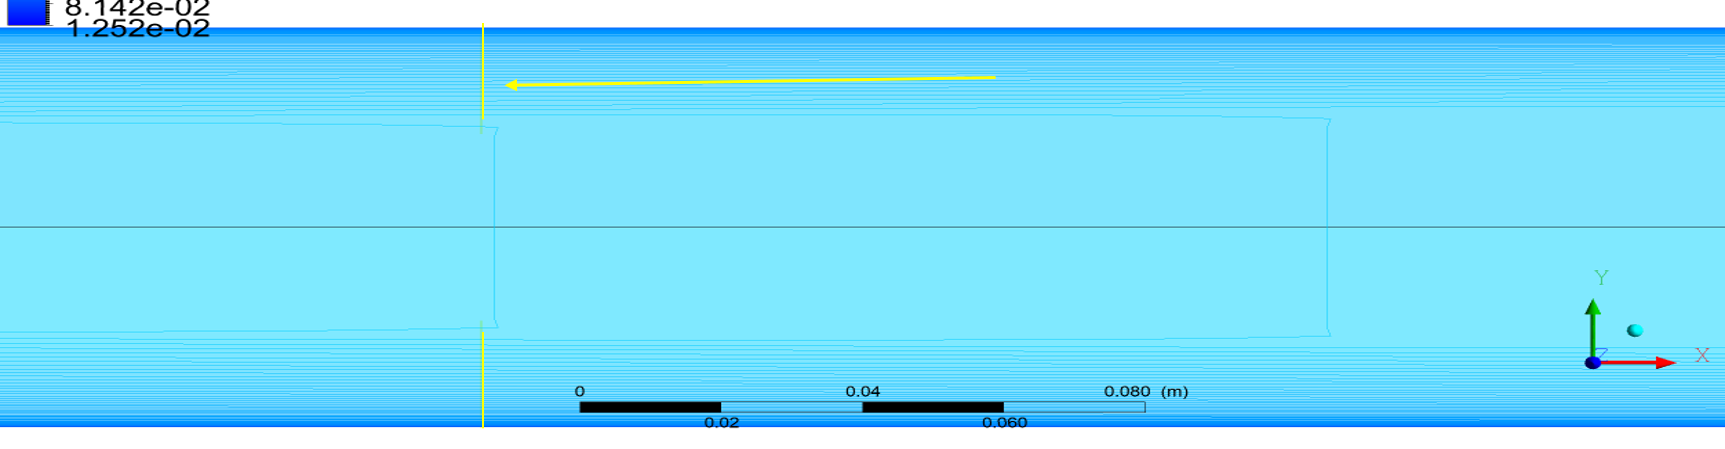
\includegraphics[width = \linewidth]{BoundaryLength.PNG}
    \captionof{figure}{CFD Post - Pipe Length}
    \label{fig:boundarylength}
\end{center}

\subsection{Meshing}\label{section:mesh}
Insert information here about meshing. To refer to meshes, use Figure \ref{fig:geomA}, \ref{fig:geomB}, and \ref{fig:geomC} for (a), (b), and (c) respectively.

\begin{center}
    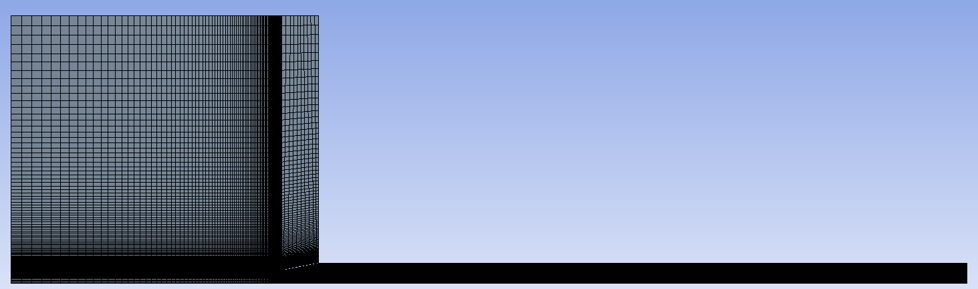
\includegraphics[width = \linewidth]{NozzleA_Mesh.PNG}
    \captionof{figure}{Nozzle (a) Coarse Mesh}
    \label{fig:geomA}
\end{center}

\begin{center}
    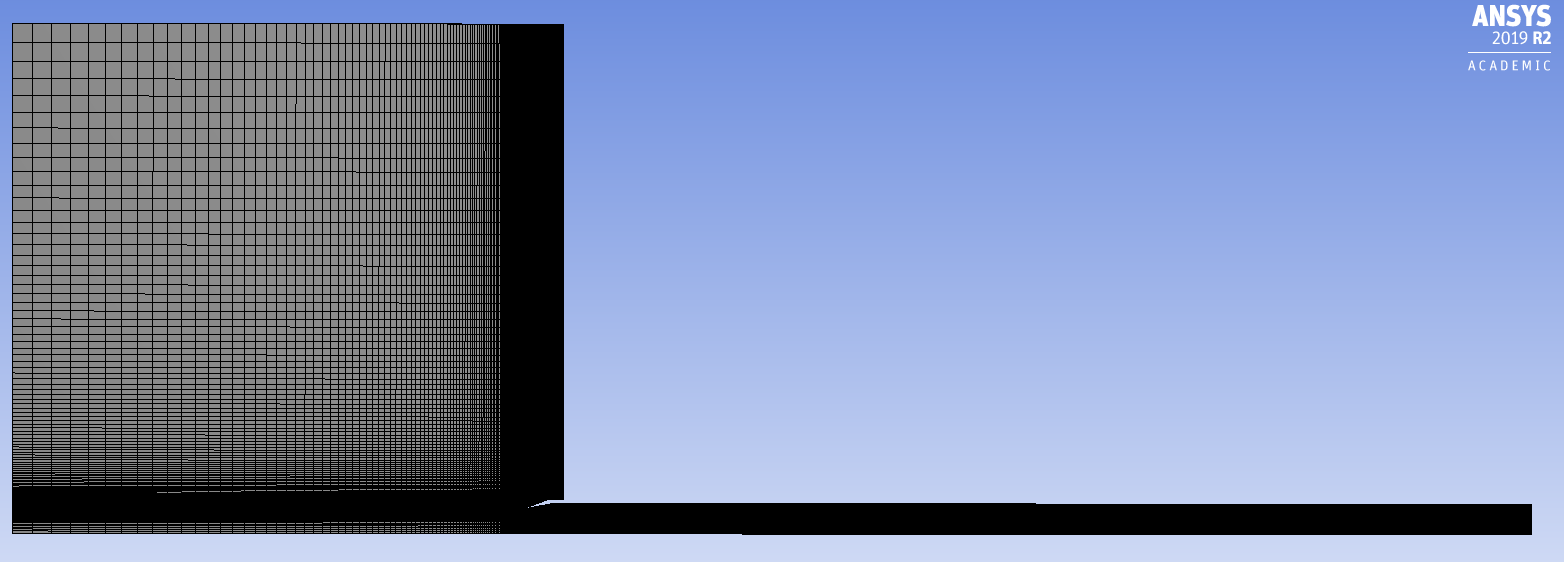
\includegraphics[width = \linewidth]{NozzleB_Mesh.PNG}
    \captionof{figure}{Nozzle (b) Coarse Mesh}
    \label{fig:geomB}
\end{center}

\begin{center}
    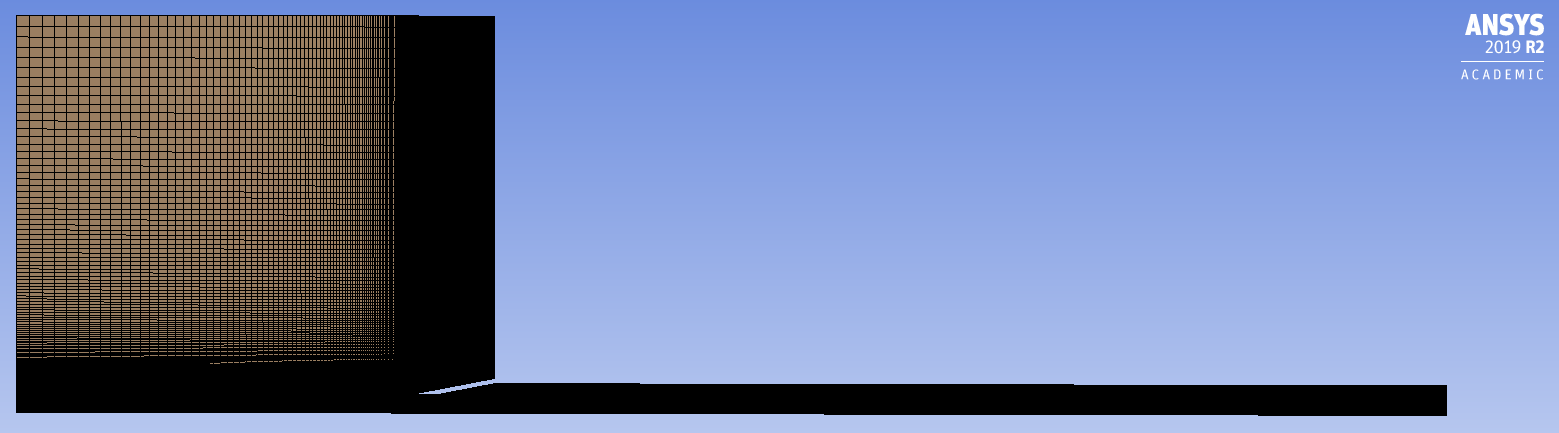
\includegraphics[width = \linewidth]{NozzleC_Mesh.PNG}
    \captionof{figure}{Nozzle (c) Coarse Mesh}
    \label{fig:geomC}
\end{center}

A grid comparison was completed on Nozzle A to ensure the aspect ratio was maintained between the coarse and fine grids. A close-up view of these grids is shown in Figure \ref{fig:gridcompareA}. The aspect ratio for the coarse grid was 252.81; the aspect ratio for the fine grid was 251.72.

\begin{center}
    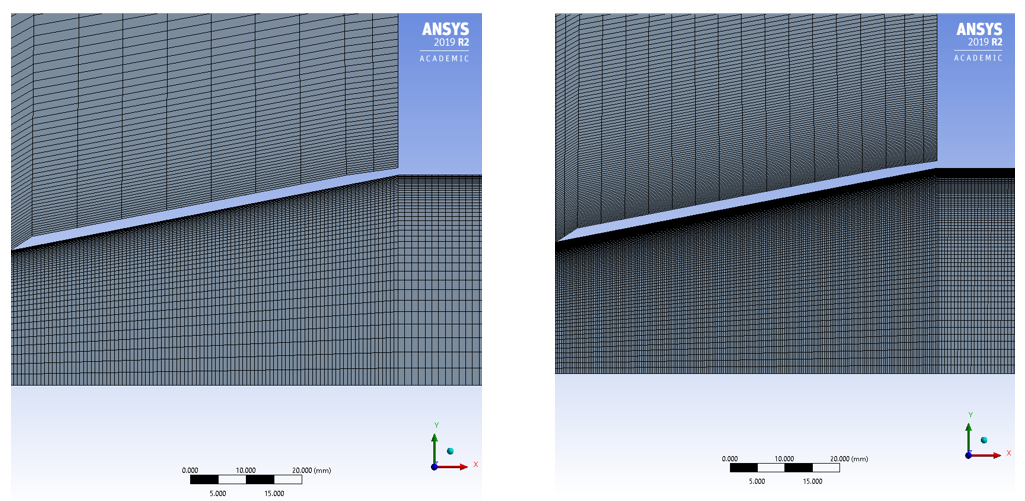
\includegraphics[width = \linewidth]{GridCompareA.png}
    \captionof{figure}{Nozzle (a) Grid Comparison}
    \label{fig:gridcompareA}
\end{center}

\begin{center}
    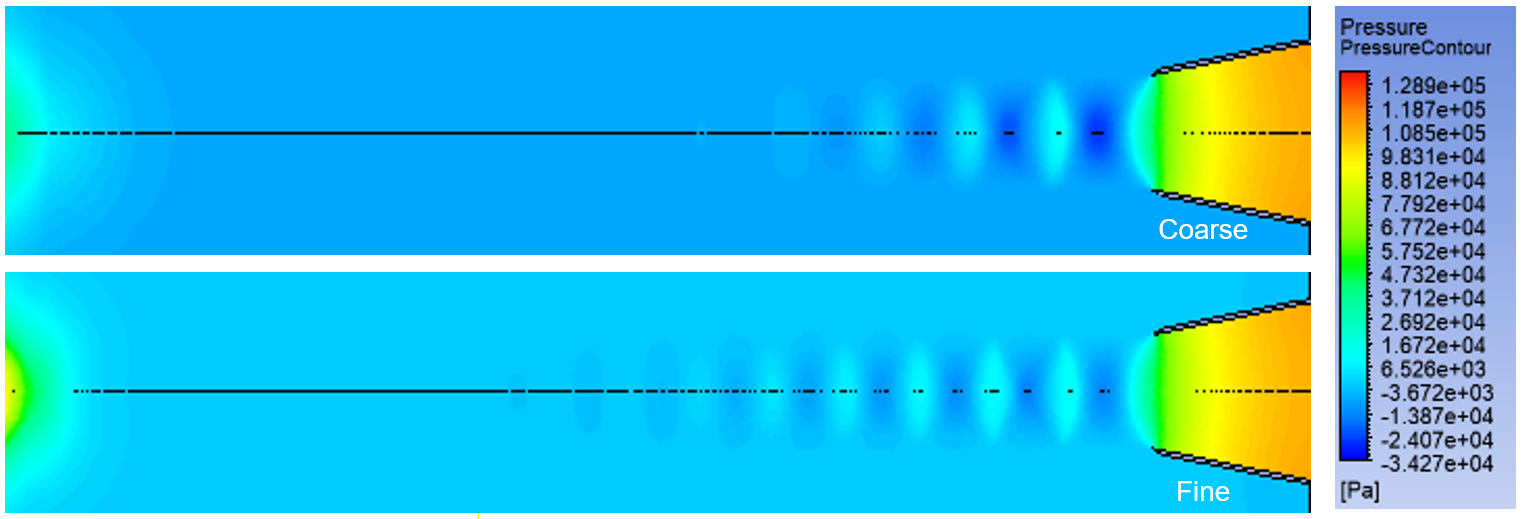
\includegraphics[width = \linewidth]{GridCompareA_Pressure.PNG}
    \captionof{figure}{Nozzle (a) Pressure Comparison}
    \label{fig:gridcompareA_Pressure}
\end{center}

\begin{center}
    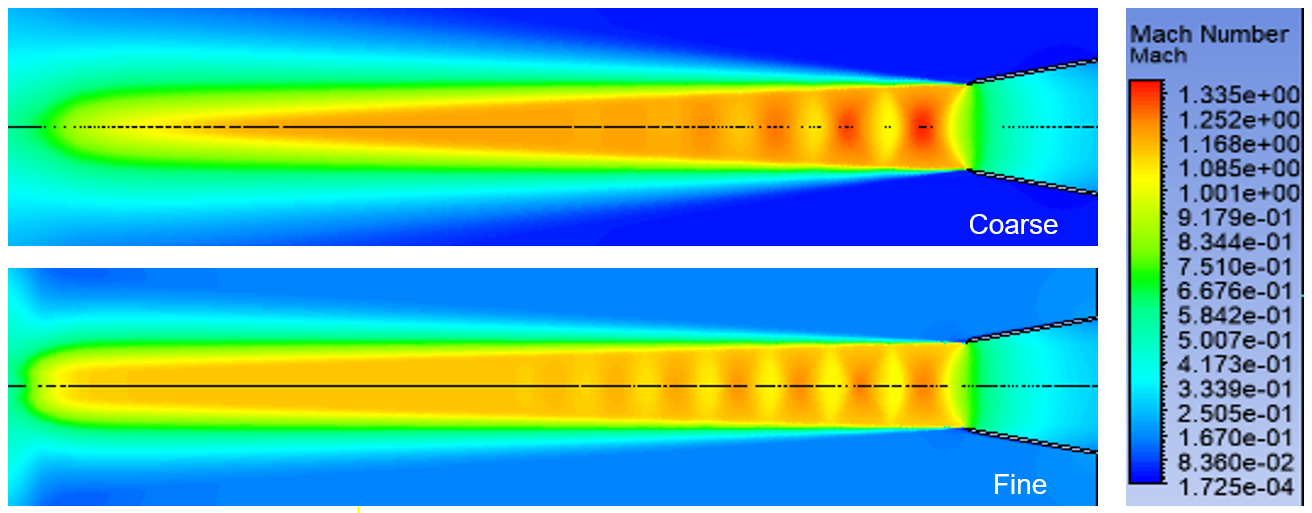
\includegraphics[width = \linewidth]{GridCompareA_Mach.PNG}
    \captionof{figure}{Nozzle (a) Mach Comparison}
    \label{fig:gridcompareA_Mach}
\end{center}

\subsection{Fluent}\label{section:fluent}
Named selections were applied to the geometries, as shown in Figure \ref{fig:namedselection}. Then, ANSYS Fluent was used to provide a CFD solution. Because the NPR used in this problem was known to create supersonic flow, a density based solver was used. Additionally, because the pipe and nozzle are round, the problem was set up with axisymmetric flow. A realizable k-\textepsilon\:model was used with a standard wall function to solve for viscosity in the flow. This model required that the fluid density be defined with an ideal gas model.

\begin{center}
    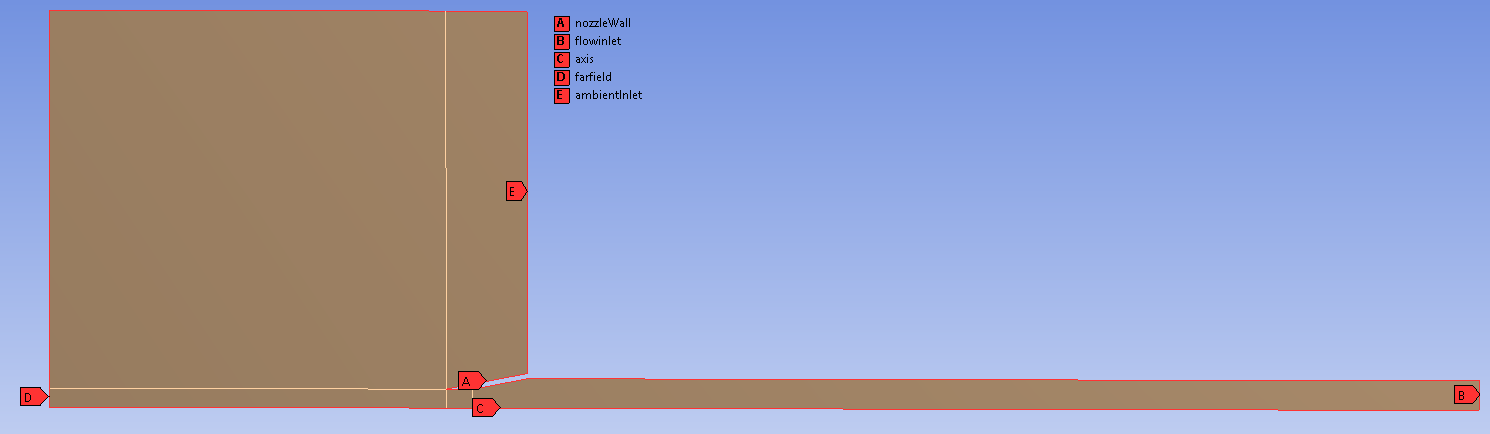
\includegraphics[width = \linewidth]{Named_Selections.PNG}
    \captionof{figure}{Named Selections}
    \label{fig:namedselection}
\end{center}

Boundary conditions, shown in Table \ref{tab:boundary}, were applied to each of the named selections. The atmospheric pressure was defined as 101,325 Pa. All of the other pressures are defined as gauge pressure.

\begin{table}[ht]
    \caption{Boundary Conditions}
    \centering
    \begin{tabular}{l|l}
        Named Selection&Boundary Condition\\
        \hline
        nozzleWall&wall\\
        farfield&pressure-far-field\\
        flowinlet&pressure-inlet\\
        ambientInlet&velocity-inlet\\
        axis&axis\\
        \hline
    \end{tabular}
    \label{tab:boundary}
\end{table}

Because the reference paper from Trumper, et al. used right-to-left flow, our geometry was set to do the same. As a result, it was required to set boundary flow velocities and Mach numbers in the negative direction. The flow inlet was defined with a gauge pressure of 121,590 Pa, matching the NPR of 2.2 as shown in Equation \ref{eq:inletpressure} below.

\begin{equation}\label{eq:inletpressure}
    p_{inlet,gauge}=\left(p_{a,total}\cdot \textnormal{NPR}\right)-p_{a,total}
\end{equation}

In order to ensure the Fluent simulation would properly define flow coming out of the nozzle, a very slight fluid motion was defined for the boundary conditions outside of the nozzle. This was done using the ambient inlet and far-field. The ambient inlet was defined with an input velocity of 10 m/s in the negative-x direction and a gauge pressure of 10 Pa. The far-field was defined with a Mach number of .1 in the negative-x direction and a gauge pressure of 20 Pa. No additional parameters were required for the axis or wall conditions. These parameters were used for each geometry on both coarse and fine grids with an explicit formulation and a Second-Order Upwind scheme to ensure a solution that was stable and accurate. To further stabilize the solution, a Courant number of 1 was used.\par

All six cases were run using the Linux servers in the Purdue University School of Aeronautics and Astronautics CAD lab. Each case was run for a minimum of 200,000 iterations. For each case, no divergence was detected and the residuals stabilized at less than $10^{-4}$.

\clearpage
\section{Results}
This is where we will write our Results Section.  (includes analysis and discussion). The pictures from the presentation are below:

\subsection{Nozzle Exit Comparison}
\begin{center}
    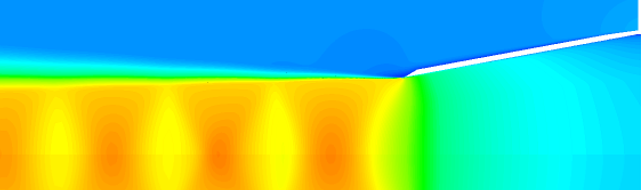
\includegraphics[width=4in]{Mach_A.png}
    \captionof{figure}{Mach Contours For Nozzle (a)}
    \label{fig:mach_A}
\end{center}

\begin{center}
    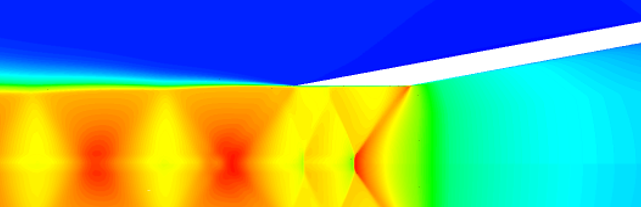
\includegraphics[width=4in]{Mach_C_Fine.png}
    \captionof{figure}{Mach Contours For Nozzle (c)}
    \label{fig:mach_C}
\end{center}

\begin{center}
    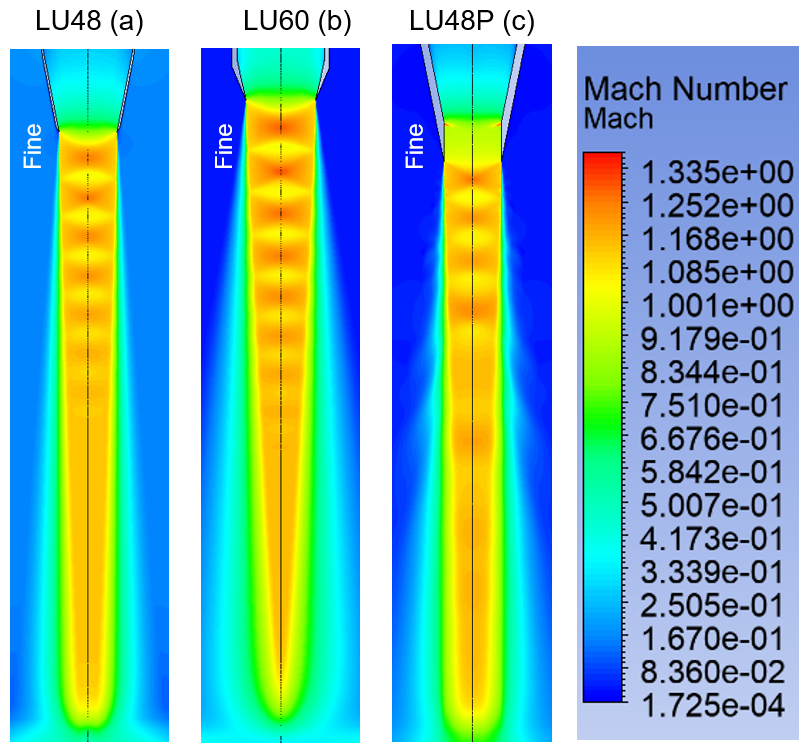
\includegraphics[width=4in]{NozzleCompare_Mach.PNG}
    \captionof{figure}{A Comparison of Nozzles (a) and (c)}
    \label{fig:NozzleComparison}
\end{center}

\begin{center}
    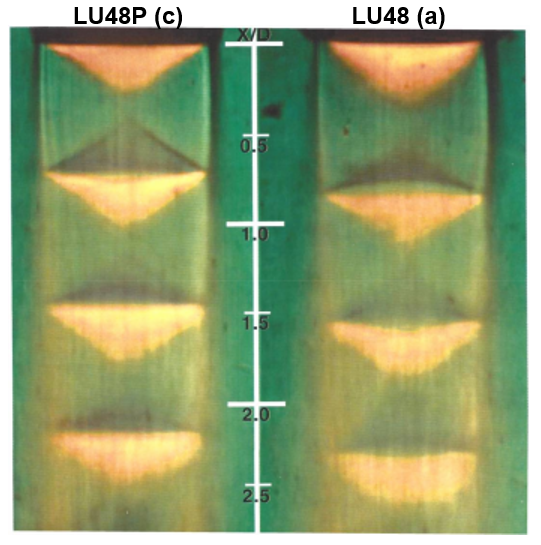
\includegraphics[width=4in]{VenaContracta_Real.PNG}
    \captionof{figure}{The Vena Contracta Effect (Actual) \cite{MilesT.Trumper2018IoNE}}
    \label{fig:VenaContractaReal}
\end{center}

\begin{center}
    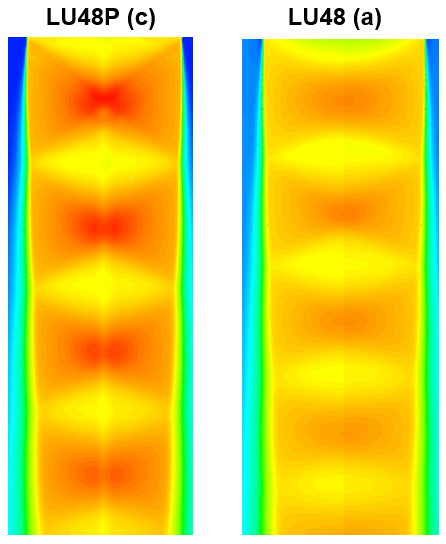
\includegraphics[width=4in]{VenaContracta_CFD.PNG}
    \captionof{figure}{The Vena Contracta Effect (Simulation)}
    \label{fig:VenaContractaCFD}
\end{center}

\subsection{Boundary Layer Analysis}
\begin{center}
    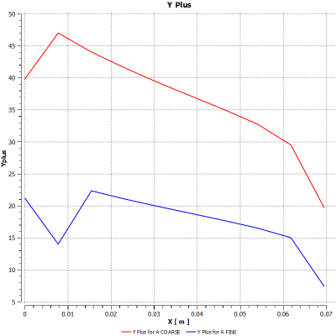
\includegraphics[width=4in]{YPlus_A.png}
    \captionof{figure}{$y^+$ For Nozzle (a)}
    \label{fig:YPlusA}
\end{center}

\begin{center}
    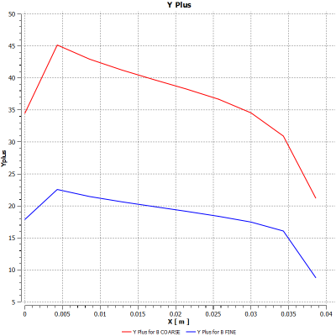
\includegraphics[width=4in]{YPlus_B.png}
    \captionof{figure}{$y^+$ For Nozzle (b)}
    \label{fig:YPlusB}
\end{center}

\begin{center}
    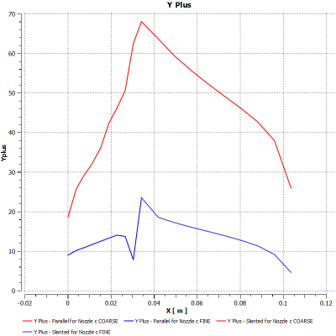
\includegraphics[width=4in]{YPlus_C.png}
    \captionof{figure}{$y^+$ For Nozzle (c)}
    \label{fig:YPlusC}
\end{center}


\subsection{Further Research: Jet Exhuast}

In looking for what to add to the CFD project to set it apart from the experiment, there was motivation to use a chemical approximation more comparable to jet exhaust. Table \ref{tab:pollution} shows that a substantial portion of jet exhaust is CO2. For this reason, it was decided that replacing the working fluid of air with C02 would be a rough estimation of running a case with jet exhaust. Nozzle A as selected to do this run as it was the most basic geometry and could be compared the most easily. Figures \ref{fig:mach_air} and \ref{fig:mach_CO2} show the Mach contours of nozzle A using air and CO2 respectively.

\begin{center}
    \captionof{table}{Pollution Emissions From Jet Aircraft \cite{lozano_melvin_ochheiser_1968}}
    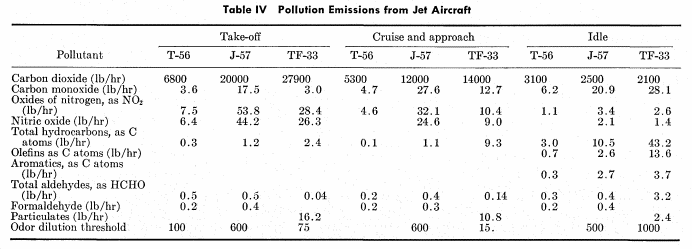
\includegraphics[width=\linewidth]{JetPollutionTable.png}
    \label{tab:pollution}
\end{center}

\begin{center}
    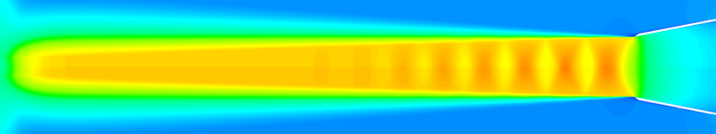
\includegraphics[width=6in]{Mach_Air.png}
    \captionof{figure}{Mach Contours for Air in Nozzle (a)}
    \label{fig:mach_air}
\end{center}

\begin{center}
    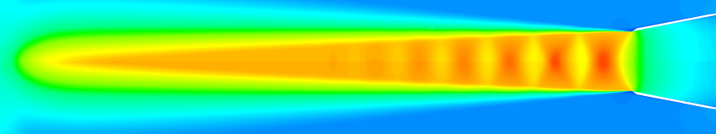
\includegraphics[width=6in]{Mach_CO2.png}
    \captionof{figure}{Mach Contours for Carbon Dioxide in Nozzle (a)}
    \label{fig:mach_CO2}
\end{center}

The largest observation from this case is the much slower flow throughout the plume. This is due to CO2 having a higher molecular mass then air, 44g/mol compared to about 29g/mol. Holding the NPR constant at 2.2 meant that the heavier fluid resulted in a lower flow velocity. The contour still shows sonic flow in the nozzle and Mach diamonds in the near field, however they are much less defined than the air’s results and decay much quicker. Interpolating this observation further suggests that without changing the NPR a heavy enough fluid could be used to a point that eventually chocked flow would no longer be seen and the flow would remain subsonic. One other observation made from these contours is the comparison of the plume shape extending out from the nozzle exits. While the flow is slower all around for the CO2, the flow profile and expansion are actually very similar to that of the air’s. This suggests that where plume shape is concerned, nozzle geometry is the important consideration and not the fluid being used.

Pressure contours are also included in <figure> to reconfirm the observations made using the velocity. Very few pockets of low pressure exist in the CO2 case compared to air which has many alternating low and high pressures extending well farther past the exit. This pattern is consistent with the nozzle’s Mach diamond pattern and reinforces the fact that the heavier CO2 results in a slower flow.

\begin{center}
    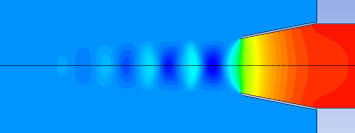
\includegraphics[width=4in]{Pressure_Air.png}
    \captionof{figure}{Pressure Contours for Air in Nozzle (a)}
    \label{fig:pressure_air}
\end{center}

\begin{center}
    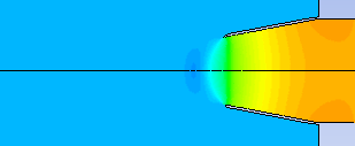
\includegraphics[width=4in]{Pressure_CO2.png}
    \captionof{figure}{Pressure Contours for Carbon Dioxide in Nozzle (a)}
    \label{fig:pressure_CO2}
\end{center}





\section{Conclusions}
This is where we will write our Conclusions Section.  (similar to the abstract, but contains a more detailed summary
of the results you found, lessons learned and suggestions for further study (if
appropriate)).
\subsection{Summary of Results}
\subsection{Lessons Learned}

\subsection{Suggestions for Further Research}
Given more time and resources there are several things that would ideally be explored in this project. The first addition that would be advantageous to have would be a more extensive grid study. This is based on the fact that the Yplus in these models dip as low as 7 in the fine grid’s case. Using k-epsilon, as was done in this project, the yplus should ideally stay between 30 and 300. With a yplus much below that there can be problems in the viscous model limiting the accuracy of the solution. Secondly, more complete encompassment of the experimental scope would offer a wider range of data to compare. While researchers in <reference> modeled 4 different geometries and an entire range of NPRs, CFD was only done on three specific cases limiting the extent of the comparisons and reliable data. Finally, refining the jet exhaust case would be a priority moving forward. Running for more geometries and with a more accurate representation of exhaust, versus just CO2, could provide a much-wanted base for analysis of jet engine nozzle design.





\section{References}
%Note: Do not change this! References are added in BibTex format in AAE412Bib.bib
This is where we will place the references
\nocite{*}
\begingroup
\renewcommand{\section}[2]{}%Remove Extra Title
\bibliographystyle{abbrv}
\bibliography{AAE412Bib}
\endgroup


\clearpage
{\Large{\color{red}Begin Useful Stuff for learning LaTeX}}

I will attempt to place a graphic in this section with a caption:
\begin{center}
\includegraphics{rootlocus.png}
\captionof{figure}{Sample Root Locus}
\end{center}

\clearpage

\section{Tables}

Coming up in the section below is a table with a caption.

\subsection{Table Subsection}

\begin{table}[ht]
\caption{Sample Table Title} % title of Table
\centering % used for centering table
\begin{tabular}{l | c c c} % a left-text column, vertical line, then 3 centered columns
\hline\hline %inserts double horizontal lines
Heading\#1 & Heading\#2 & Heading\#3 & Heading\#4 \\ [0.5ex] % inserts table
%heading
\hline % inserts single horizontal line
1 & 50 & 837 & 970 \\ % inserting body of the table
2 & 47 & 877 & 230 \\
3 & 31 & 25 & 415 \\
4 & 35 & 144 & 2356 \\
5 & 45 & 300 & 556 \\ [1ex] % [1ex] adds vertical space
\hline %inserts single line
\end{tabular}
\label{table:nonlin} % is used to refer this table in the text
\end{table}

\clearpage

\section{Equations}

This subsection will have equations that are numbered

\subsection{Equations below!}

%Equations with numbering
\begin{align}
1\:+\:k_iL\left(j\omega \right)\:=\:0\\
                          &= 0
\end{align} 

%Equations with no numbering in specific line by using \nonumber
\begin{align}
L\left(s\right)\:=\:\frac{\gamma }{m\left(j\omega \right)^3+c\left(j\omega \right)^2+\gamma \left(j\omega \right)}\nonumber\\
\end{align}

%Equations without numbering
\begin{align*}
j\omega \left(17.24\:-\:7.031\omega^2\right)+\left(1.7235k_i-11.79\omega ^2\right)\:=\:0
\end{align*} 

Of course, math can still be placed using inline text, like this $1.7235k_i\:=\:11.79\omega ^2\:=28.9091$

\clearpage

%Convert to the APPENDIX Portion of the document using the next two lines. 
\appendixpage
\appendix

Appendicies are here

\end{document}
